% metodos.tex
\section{Métodos}\label{sec:metodos}

\subsection{Patrón Bayer RGGB}

El patrón Bayer RGGB organiza los filtros de color en una matriz donde:
\begin{itemize}
    \item Las filas pares comienzan con rojo (R) y verde (G) alternados
    \item Las filas impares comienzan con verde (G) y azul (B) alternados
\end{itemize}

\begin{figure}[h]
\centering
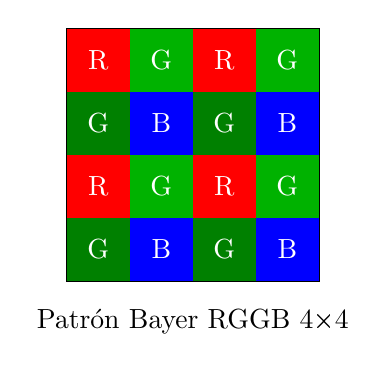
\begin{tikzpicture}[scale=0.8]
    % Cuadrícula 4x4
    \draw[gray!30, very thin] (0,0) grid (4,4);
    \draw[black, thick] (0,0) rectangle (4,4);
    
    % Fila 1: R G R G
    \fill[red] (0,3) rectangle (1,4);
    \fill[green!70!black] (1,3) rectangle (2,4);
    \fill[red] (2,3) rectangle (3,4);
    \fill[green!70!black] (3,3) rectangle (4,4);
    
    % Fila 2: G B G B
    \fill[green!50!black] (0,2) rectangle (1,3);
    \fill[blue] (1,2) rectangle (2,3);
    \fill[green!50!black] (2,2) rectangle (3,3);
    \fill[blue] (3,2) rectangle (4,3);
    
    % Fila 3: R G R G
    \fill[red] (0,1) rectangle (1,2);
    \fill[green!70!black] (1,1) rectangle (2,2);
    \fill[red] (2,1) rectangle (3,2);
    \fill[green!70!black] (3,1) rectangle (4,2);
    
    % Fila 4: G B G B
    \fill[green!50!black] (0,0) rectangle (1,1);
    \fill[blue] (1,0) rectangle (2,1);
    \fill[green!50!black] (2,0) rectangle (3,1);
    \fill[blue] (3,0) rectangle (4,1);
    
    % Etiquetas
    \node[white] at (0.5,3.5) {R};
    \node[white] at (1.5,3.5) {G};
    \node[white] at (2.5,3.5) {R};
    \node[white] at (3.5,3.5) {G};
    
    \node[white] at (0.5,2.5) {G};
    \node[white] at (1.5,2.5) {B};
    \node[white] at (2.5,2.5) {G};
    \node[white] at (3.5,2.5) {B};
    
    \node[white] at (0.5,1.5) {R};
    \node[white] at (1.5,1.5) {G};
    \node[white] at (2.5,1.5) {R};
    \node[white] at (3.5,1.5) {G};
    
    \node[white] at (0.5,0.5) {G};
    \node[white] at (1.5,0.5) {B};
    \node[white] at (2.5,0.5) {G};
    \node[white] at (3.5,0.5) {B};
    
    \node[below] at (2,-0.3) {Patrón Bayer RGGB 4×4};
\end{tikzpicture}
\caption{Distribución de canales en patrón Bayer RGGB}
\end{figure}

\subsection{Interpolación Lineal}
La interpolación lineal es el método más simple, usando el promedio de vecinos inmediatos:

\[
P_{\text{interp}} = \frac{\sum^{K}_{k=1} P_k}{K}
\]

% demosaicado_bilineal_tikz.tex
% Gráfica TikZ del proceso de demosaicado bilineal - Versión corregida con superposición de esquinas

\begin{figure}[h]
\centering
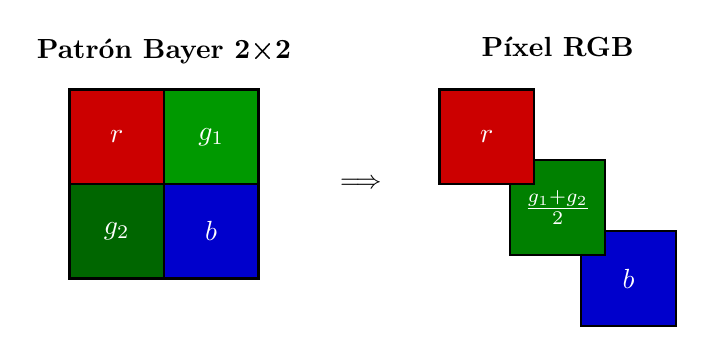
\begin{tikzpicture}[
    font=\small,
    pixel/.style={rectangle, draw=black, minimum width=1.2cm, minimum height=1.2cm, inner sep=0}
]

% ============================================
% PATRÓN BAYER ORIGINAL (2x2 RGGB)
% ============================================

% Cuadrante superior izquierdo (rojo)
\fill[red!80!black] (-1.2,0) rectangle (0,1.2);
\draw[black, thick] (-1.2,0) rectangle (0,1.2);
\node[white, font=\bfseries] at (-0.6,0.6) (r) {$r$};

% Cuadrante superior derecho (verde 1)
\fill[green!60!black] (0,0) rectangle (1.2,1.2);
\draw[black, thick] (0,0) rectangle (1.2,1.2);
\node[white, font=\bfseries] at (0.6,0.6) (g1) {$g_1$};

% Cuadrante inferior izquierdo (verde 2)
\fill[green!40!black] (-1.2,-1.2) rectangle (0,0);
\draw[black, thick] (-1.2,-1.2) rectangle (0,0);
\node[white, font=\bfseries] at (-0.6,-0.6) (g2) {$g_2$};

% Cuadrante inferior derecho (azul)
\fill[blue!80!black] (0,-1.2) rectangle (1.2,0);
\draw[black, thick] (0,-1.2) rectangle (1.2,0);
\node[white, font=\bfseries] at (0.6,-0.6) (b) {$b$};

% Marco exterior del patrón
\draw[black, very thick] (-1.2,-1.2) rectangle (1.2,1.2);

% Título
\node[above, align=center, font=\bfseries] at (0,1.4) 
    {Patrón Bayer 2×2};

% ============================================
% FLECHA DE PROCESO
% ============================================
\node at (2.5,0) {$\Longrightarrow$};

% ============================================
% PÍXEL RESULTANTE (CARTAS SUPERPUESTAS CON ESQUINAS)
% ============================================

% Parámetros
\def\cardsize{1.2cm}
\def\overlap{0.3cm} % L/4 = 1.2cm/4 = 0.3cm
\def\shift{0.9cm} % cardsize - overlap = 1.2 - 0.3 = 0.9cm
\def\sqareorigin{3.5cm}

% ORDEN: Primero dibujamos la de atrás (B), luego la del medio (G), luego la del frente (R)

% Azul (B) - atrás - más desplazada hacia abajo y derecha
\fill[blue!80!black]                (\sqareorigin+2*\shift            , -2*\shift) rectangle (\sqareorigin+2*\shift+\cardsize, -2*\shift+\cardsize);
\draw[black, thick]                 (\sqareorigin+2*\shift            , -2*\shift) rectangle (\sqareorigin+2*\shift+\cardsize, -2*\shift+\cardsize);
\node[white, font=\bfseries] at     (\sqareorigin+2*\shift+\cardsize/2, -2*\shift+\cardsize/2) (B) {$b$};

% Verde (G) - medio - desplazada un shift
\fill[green!50!black]               (\sqareorigin+\shift              , -  \shift) rectangle (\sqareorigin+\shift+\cardsize, -\shift+\cardsize);
\draw[black, thick]                 (\sqareorigin+\shift              , -  \shift) rectangle (\sqareorigin+\shift+\cardsize, -\shift+\cardsize);
\node[white, font=\bfseries] at     (\sqareorigin+\shift+\cardsize/2  , -  \shift+\cardsize/2) (G) {$\frac{g_1 + g_2}{2}$};

% Rojo (R) - frente - posición base (sin desplazar)
\fill[red!80!black]                 (\sqareorigin,0) rectangle (\sqareorigin+\cardsize           , \cardsize);
\draw[black, thick]                 (\sqareorigin,0) rectangle (\sqareorigin+\cardsize           , \cardsize);
\node[white, font=\bfseries] at     (\sqareorigin+\cardsize/2         , \cardsize/2) (R) {$r$};

% Título del píxel resultante
\node[above, font=\bfseries] at (\sqareorigin+\cardsize/2+\shift, 1.5) {Píxel RGB};

\end{tikzpicture}
\caption{Proceso de demosaicado bilineal para patrón Bayer RGGB. Los canales de color se superponen para formar el píxel RGB final.}
\label{fig:demosaicado_bilineal}
\end{figure}


\subsection{Interpolación Bicuadrada}
Utiliza tres puntos para ajustar una parábola:

\[
P(x) = ax^2 + bx + c
\]

Para puntos equidistantes en $x \in \{-2, 0, 2\}$ (separados por 2 unidades, como en el patrón Bayer), la fórmula de interpolación para el punto intermedio en $x=1$ es:

\[
P(1) = \frac{3}{8}P(-2) + \frac{3}{4}P(0) - \frac{1}{8}P(2)
\]

En coordenadas de imagen, para el canal rojo en posición $(2k,j)$:

\[
R_{2k,j} = \frac{3}{8}R_{2k-2,j} + \frac{3}{4}R_{2k,j} - \frac{1}{8}R_{2k+2,j}
\]

% separacion_canales_bayer_tikz.tex
% Gráfica TikZ de la separación de canales en patrón Bayer - Versión exacta

\begin{figure}[h]
\centering
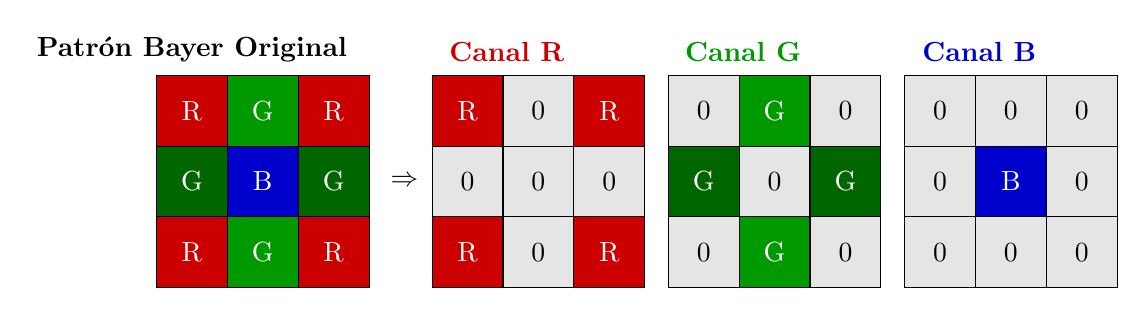
\begin{tikzpicture}[
    font=\normalsize,
    cell/.style={rectangle, draw=black, minimum size=0.9cm, inner sep=0}
]

% ============================================
% PATRÓN BAYER ORIGINAL 3×3
% ============================================

% Título
\node[above, font=\bfseries] at (0, 2.5) {Patrón Bayer Original};

% Fila 1: R G R
\node[cell, fill=red!80!black] at (0, 2) {\textcolor{white}{R}};
\node[cell, fill=green!60!black] at (0.9, 2) {\textcolor{white}{G}};
\node[cell, fill=red!80!black] at (1.8, 2) {\textcolor{white}{R}};

% Fila 2: G B G
\node[cell, fill=green!40!black] at (0, 1.1) {\textcolor{white}{G}};
\node[cell, fill=blue!80!black] at (0.9, 1.1) {\textcolor{white}{B}};
\node[cell, fill=green!40!black] at (1.8, 1.1) {\textcolor{white}{G}};

% Fila 3: R G R
\node[cell, fill=red!80!black] at (0, 0.2) {\textcolor{white}{R}};
\node[cell, fill=green!60!black] at (0.9, 0.2) {\textcolor{white}{G}};
\node[cell, fill=red!80!black] at (1.8, 0.2) {\textcolor{white}{R}};

% ============================================
% FLECHA DE SEPARACIÓN
% ============================================
\node at (2.7, 1.1) {$\Rightarrow$};

% ============================================
% CANAL ROJO (R)
% ============================================

% Título
\node[above, font=\bfseries, red!80!black] at (4, 2.5) {Canal R};

% Fila 1: R 0 R
\node[cell, fill=red!80!black] at (3.5, 2) {\textcolor{white}{R}};
\node[cell, fill=gray!20] at (4.4, 2) {0};
\node[cell, fill=red!80!black] at (5.3, 2) {\textcolor{white}{R}};

% Fila 2: 0 0 0
\node[cell, fill=gray!20] at (3.5, 1.1) {0};
\node[cell, fill=gray!20] at (4.4, 1.1) {0};
\node[cell, fill=gray!20] at (5.3, 1.1) {0};

% Fila 3: R 0 R
\node[cell, fill=red!80!black] at (3.5, 0.2) {\textcolor{white}{R}};
\node[cell, fill=gray!20] at (4.4, 0.2) {0};
\node[cell, fill=red!80!black] at (5.3, 0.2) {\textcolor{white}{R}};

% ============================================
% CANAL VERDE (G)
% ============================================

% Título
\node[above, font=\bfseries, green!60!black] at (7, 2.5) {Canal G};

% Fila 1: 0 G 0
\node[cell, fill=gray!20] at (6.5, 2) {0};
\node[cell, fill=green!60!black] at (7.4, 2) {\textcolor{white}{G}};
\node[cell, fill=gray!20] at (8.3, 2) {0};

% Fila 2: G 0 G
\node[cell, fill=green!40!black] at (6.5, 1.1) {\textcolor{white}{G}};
\node[cell, fill=gray!20] at (7.4, 1.1) {0};
\node[cell, fill=green!40!black] at (8.3, 1.1) {\textcolor{white}{G}};

% Fila 3: 0 G 0
\node[cell, fill=gray!20] at (6.5, 0.2) {0};
\node[cell, fill=green!60!black] at (7.4, 0.2) {\textcolor{white}{G}};
\node[cell, fill=gray!20] at (8.3, 0.2) {0};

% ============================================
% CANAL AZUL (B)
% ============================================

% Título
\node[above, font=\bfseries, blue!80!black] at (10, 2.5) {Canal B};

% Fila 1: 0 0 0
\node[cell, fill=gray!20] at (9.5, 2) {0};
\node[cell, fill=gray!20] at (10.4, 2) {0};
\node[cell, fill=gray!20] at (11.3, 2) {0};

% Fila 2: 0 B 0
\node[cell, fill=gray!20] at (9.5, 1.1) {0};
\node[cell, fill=blue!80!black] at (10.4, 1.1) {\textcolor{white}{B}};
\node[cell, fill=gray!20] at (11.3, 1.1) {0};

% Fila 3: 0 0 0
\node[cell, fill=gray!20] at (9.5, 0.2) {0};
\node[cell, fill=gray!20] at (10.4, 0.2) {0};
\node[cell, fill=gray!20] at (11.3, 0.2) {0};

\end{tikzpicture}
\caption{Separación de canales en patrón Bayer 3×3. El patrón original se descompone en tres matrices que muestran la información de cada canal por separado. Los ceros (gris) indican ausencia de información en esa posición para el canal correspondiente.}
\label{fig:separacion_canales_bayer}
\end{figure}

% interpolacion_bicuadrada_R_completo_tikz.tex
% Figura completa de interpolación bicuadrada para canal R (fórmulas con espaciado uniforme)

\begin{figure}[H]
\centering
\begin{tikzpicture}[
    font=\normalsize,
    cell/.style={rectangle, draw=black, minimum size=1.2cm, inner sep=0},
    legendcell/.style={rectangle, draw=black, minimum size=0.8cm, inner sep=0},
    formula/.style={font=\footnotesize, align=left}
]

% ============================================
% PARÁMETROS DE LA CUADRÍCULA
% ============================================
\def\gridWidth{14}   % Ancho total aumentado (en cm)
\def\rowOneHeight{3.5}  % Alto de la fila 1 (en cm)
\def\rowTwoHeight{3}    % Alto de la fila 2 (en cm)
\def\colWidth{2.8}    % Ancho de cada columna (en cm)

% ============================================
% DEFINICIÓN DE COORDENADAS DE CENTRO
% ============================================
% Fila 1 (ahora con 5 columnas para más espacio)
\coordinate (F1C1) at (0.5*\colWidth, 0);
\coordinate (F1C2) at (1.5*\colWidth, 0);
\coordinate (F1C3) at (2.5*\colWidth, 0);
\coordinate (F1C4) at (3.5*\colWidth, 0); % Espacio extra
\coordinate (F1C5) at (4.5*\colWidth, 0); % Leyenda más a la derecha

% Fila 2 (ocupa ancho completo de 5 columnas)
\coordinate (F2) at (2.5*\colWidth, -\rowOneHeight-0.5*\rowTwoHeight);

% ============================================
% F1C1: MATRIZ ORIGINAL - CANAL R
% ============================================
\begin{scope}[shift={(F1C1)}]
    % Título
    \node[above, font=\bfseries, red!80!black] at (0, 1.8) {Canal R Original};
    
    % Matriz 3x3
    % Fila 1
    \node[cell, fill=red!80!black] at (-1.2, 1.2) {\textcolor{white}{$r_{11}$}};
    \node[cell, fill=gray!20] at (0, 1.2) {$0$};
    \node[cell, fill=red!80!black] at (1.2, 1.2) {\textcolor{white}{$r_{13}$}};
    
    % Fila 2
    \node[cell, fill=gray!20] at (-1.2, 0) {$0$};
    \node[cell, fill=gray!20] at (0, 0) {$0$};
    \node[cell, fill=gray!20] at (1.2, 0) {$0$};
    
    % Fila 3
    \node[cell, fill=red!80!black] at (-1.2, -1.2) {\textcolor{white}{$r_{31}$}};
    \node[cell, fill=gray!20] at (0, -1.2) {$0$};
    \node[cell, fill=red!80!black] at (1.2, -1.2) {\textcolor{white}{$r_{33}$}};
\end{scope}

% ============================================
% F1C2: FLECHA DE PROCESO
% ============================================
\begin{scope}[shift={(F1C2)}]
    \node[font=\Huge] at (0, 0) {$\Rightarrow$};
    \node[above, font=\scriptsize] at (0, 1) {Interpolación};
    \node[below, font=\scriptsize] at (0, -1) {Bicuadrada};
\end{scope}

% ============================================
% F1C3: MATRIZ INTERPOLADA - CANAL R
% ============================================
\begin{scope}[shift={(F1C3)}]
    % Título
    \node[above, font=\bfseries, red!80!black] at (0, 1.8) {Canal R Interpolado};
    
    % Matriz 3x3 completa
    % Fila 1
    \node[cell, fill=red!80!black] at (-1.2, 1.2) {\textcolor{white}{$r_{11}$}};
    \node[cell, fill=red!60!black] at (0, 1.2) {\textcolor{white}{$r_{12}$}};
    \node[cell, fill=red!80!black] at (1.2, 1.2) {\textcolor{white}{$r_{13}$}};
    
    % Fila 2
    \node[cell, fill=red!60!black] at (-1.2, 0) {\textcolor{white}{$r_{21}$}};
    \node[cell, fill=red!40!black] at (0, 0) {\textcolor{white}{$r_{22}$}};
    \node[cell, fill=red!60!black] at (1.2, 0) {\textcolor{white}{$r_{23}$}};
    
    % Fila 3
    \node[cell, fill=red!80!black] at (-1.2, -1.2) {\textcolor{white}{$r_{31}$}};
    \node[cell, fill=red!60!black] at (0, -1.2) {\textcolor{white}{$r_{32}$}};
    \node[cell, fill=red!80!black] at (1.2, -1.2) {\textcolor{white}{$r_{33}$}};
\end{scope}

% ============================================
% F1C5: LEYENDA DE COLORES (AJUSTADA VERTICALMENTE)
% ============================================
\begin{scope}[shift={(F1C5)}]
    % Título
    \node[above, font=\bfseries] at (0, 1.8) {Leyenda de Colores};
    
    % Ajuste: movemos toda la leyenda 0.8cm hacia arriba
    \def\verticalShift{0.8}
    
    % Original (rojo oscuro)
    \node[legendcell, fill=red!80!black] at (-1, 0.5+\verticalShift) {};
    \node[anchor=west, font=\small] at (-0.7, 0.5+\verticalShift) {Original};
    \node[anchor=west, font=\tiny] at (-0.7, 0.2+\verticalShift) {($r_{11}$, $r_{13}$, $r_{31}$, $r_{33}$)};
    
    % Interpolado 1D (rojo medio)
    \node[legendcell, fill=red!60!black] at (-1, -0.3+\verticalShift) {};
    \node[anchor=west, font=\small] at (-0.7, -0.3+\verticalShift) {Interpolado 1D};
    \node[anchor=west, font=\tiny] at (-0.7, -0.6+\verticalShift) {($r_{12}$, $r_{21}$, $r_{23}$, $r_{32}$)};
    
    % Interpolado 2D (rojo claro)
    \node[legendcell, fill=red!40!black] at (-1, -1.1+\verticalShift) {};
    \node[anchor=west, font=\small] at (-0.7, -1.1+\verticalShift) {Interpolado 2D};
    \node[anchor=west, font=\tiny] at (-0.7, -1.4+\verticalShift) {($r_{22}$)};
    
    % Por interpolar (gris)
    \node[legendcell, fill=gray!20] at (-1, -1.9+\verticalShift) {};
    \node[anchor=west, font=\small] at (-0.7, -1.9+\verticalShift) {Por interpolar};
    \node[anchor=west, font=\tiny] at (-0.7, -2.2+\verticalShift) {(valor 0)};
\end{scope}

% ============================================
% F2: FÓRMULAS DE INTERPOLACIÓN CON ESPACIADO UNIFORME
% ============================================
\begin{scope}[shift={(F2)}]
    % Título
    \node[above, font=\bfseries] at (0, 1.5) {Fórmulas de Interpolación Bicuadrada};
    
    % Parámetros para el espaciado uniforme
    \def\formulaStartY{0.8}      % Coordenada Y inicial
    \def\formulaSpacing{0.7}     % Espaciado uniforme entre fórmulas
    \def\leftColumnX{-4}         % Columna izquierda
    \def\rightColumnX{2}         % Columna derecha (separada 6cm de la izquierda)
    
    % Columna izquierda: 3 fórmulas
    \node[anchor=north west, formula] at (\leftColumnX, \formulaStartY) 
        {$r_{12} = \tfrac{3}{8}r_{11} + \tfrac{3}{4}r_{13} - \tfrac{1}{8}r_{15}$};
    
    \node[anchor=north west, formula] at (\leftColumnX, \formulaStartY - \formulaSpacing) 
        {$r_{21} = \tfrac{3}{8}r_{11} + \tfrac{3}{4}r_{31} - \tfrac{1}{8}r_{51}$};
    
    \node[anchor=north west, formula] at (\leftColumnX, \formulaStartY - 2*\formulaSpacing) 
        {$r_{22} = \tfrac{9}{64}r_{11} + \tfrac{9}{32}r_{13} + \tfrac{9}{32}r_{31} + \tfrac{9}{16}r_{33} - \tfrac{3}{64}r_{15} - \tfrac{3}{64}r_{51}$};
    
    % Columna derecha: 2 fórmulas (alineadas con las dos primeras de la izquierda)
    \node[anchor=north west, formula] at (\rightColumnX, \formulaStartY) 
        {$r_{23} = \tfrac{3}{8}r_{13} + \tfrac{3}{4}r_{33} - \tfrac{1}{8}r_{53}$};
    
    \node[anchor=north west, formula] at (\rightColumnX, \formulaStartY - \formulaSpacing) 
        {$r_{32} = \tfrac{3}{8}r_{31} + \tfrac{3}{4}r_{33} - \tfrac{1}{8}r_{35}$};
    
    % Línea vertical divisoria (opcional, para referencia)
    \draw[gray!30, dashed] (\leftColumnX + 3, \formulaStartY + 0.2) -- (\leftColumnX + 3, \formulaStartY - 2*\formulaSpacing - 0.2);
\end{scope}

% ============================================
% LÍNEA DIVISORIA HORIZONTAL
% ============================================
\draw[gray!40, thick] (0.2, -\rowOneHeight+0.2) -- (\gridWidth-0.2, -\rowOneHeight+0.2);

\end{tikzpicture}
\caption{Interpolación bicuadrada para el canal rojo (R) en patrón Bayer. Arriba se muestra la transformación de la matriz original (con valores conocidos en rojo oscuro y ceros en gris) a la matriz interpolada (todos los valores completos, diferenciando entre originales, interpolados 1D e interpolados 2D). La leyenda, alineada verticalmente con las matrices, explica los colores utilizados. Debajo se presentan las fórmulas de interpolación bicuadrada con espaciado uniforme, distribuidas en dos columnas para una presentación clara y ordenada.}
\label{fig:interpolacion_bicuadrada_R_completa}
\end{figure}


\subsection{Interpolación Bicúbica}
Utiliza cuatro puntos para ajustar un polinomio cúbico:

\[
P(x) = ax^3 + bx^2 + cx + d
\]

Con puntos en $x \in \{-2, 0, 2, 4\}$, usando el kernel cúbico de Catmull-Rom:

\[
P(1) = -\frac{1}{16}P(-2) + \frac{9}{16}P(0) + \frac{9}{16}P(2) - \frac{1}{16}P(4)
\]

Para el canal verde en posición $(2k+1,2\ell)$:

\[
G_{2k+1,2\ell} = -\frac{1}{16}G_{2k-3,2\ell} + \frac{9}{16}G_{2k-1,2\ell} + \frac{9}{16}G_{2k+3,2\ell} - \frac{1}{16}G_{2k+5,2\ell}
\]

% interpolacion_bicubica_R_completo_tikz_final5.tex
% Versión final con fórmulas más a la izquierda y títulos separados

\begin{figure}[h]
\centering
\begin{tikzpicture}[
    font=\normalsize,
    cell/.style={rectangle, draw=black, minimum size=0.9cm, inner sep=0},
    legendcell/.style={rectangle, draw=black, minimum size=0.8cm, inner sep=0},
    formula/.style={font=\footnotesize, align=left}
]

% ============================================
% PARÁMETROS DE LA CUADRÍCULA
% ============================================
\def\gridWidth{16}   % Ancho total aumentado (en cm)
\def\rowOneHeight{3.5}  % Alto de la fila 1 (en cm)
\def\rowTwoHeight{5.0}  % Alto de la fila 2 reducido (en cm)
\def\colWidth{2.8}    % Ancho de cada columna (en cm)

% ============================================
% DEFINICIÓN DE COORDENADAS DE CENTRO
% ============================================
% Fila 1 (5 columnas)
\coordinate (F1C1) at (0.5*\colWidth, 0);
\coordinate (F1C2) at (1.5*\colWidth, 0);
\coordinate (F1C3) at (2.5*\colWidth, 0);
\coordinate (F1C4) at (3.5*\colWidth, 0);
\coordinate (F1C5) at (4.5*\colWidth, 0);

% Fila 2 (ocupa ancho completo)
\coordinate (F2) at (2.5*\colWidth, -\rowOneHeight-0.5*\rowTwoHeight);

% ============================================
% F1C1: MATRIZ ORIGINAL - CANAL R (4×4) CORREGIDA
% ============================================
\begin{scope}[shift={(F1C1)}]
    % Título
    \node[above, font=\bfseries, red!80!black] at (0, 2.2) {Canal R Original (4×4)};
    
    % Matriz 4x4 con valores en posiciones correctas según patrón Bayer
    % Fila 1 (índice 1)
    \node[cell, fill=red!80!black] at (-1.35, 1.35) {\textcolor{white}{$r_{11}$}};
    \node[cell, fill=gray!20] at (-0.45, 1.35) {$0$};
    \node[cell, fill=red!80!black] at (0.45, 1.35) {\textcolor{white}{$r_{13}$}};
    \node[cell, fill=gray!20] at (1.35, 1.35) {$0$};
    
    % Fila 2 (índice 2)
    \node[cell, fill=gray!20] at (-1.35, 0.45) {$0$};
    \node[cell, fill=gray!20] at (-0.45, 0.45) {$0$};
    \node[cell, fill=gray!20] at (0.45, 0.45) {$0$};
    \node[cell, fill=gray!20] at (1.35, 0.45) {$0$};
    
    % Fila 3 (índice 3)
    \node[cell, fill=red!80!black] at (-1.35, -0.45) {\textcolor{white}{$r_{31}$}};
    \node[cell, fill=gray!20] at (-0.45, -0.45) {$0$};
    \node[cell, fill=red!80!black] at (0.45, -0.45) {\textcolor{white}{$r_{33}$}};
    \node[cell, fill=gray!20] at (1.35, -0.45) {$0$};
    
    % Fila 4 (índice 4)
    \node[cell, fill=gray!20] at (-1.35, -1.35) {$0$};
    \node[cell, fill=gray!20] at (-0.45, -1.35) {$0$};
    \node[cell, fill=gray!20] at (0.45, -1.35) {$0$};
    \node[cell, fill=gray!20] at (1.35, -1.35) {$0$};
\end{scope}

% ============================================
% F1C2: FLECHA DE PROCESO
% ============================================
\begin{scope}[shift={(F1C2)}]
    \node[font=\Huge] at (0, 0) {$\Rightarrow$};
    \node[above, font=\scriptsize] at (0, 1) {Interpolación};
    \node[below, font=\scriptsize] at (0, -1) {Bicúbica};
\end{scope}

% ============================================
% F1C3: MATRIZ INTERPOLADA - CANAL R (4×4)
% ============================================
\begin{scope}[shift={(F1C3)}]
    % Título
    \node[above, font=\bfseries, red!80!black] at (0, 2.2) {Canal R Interpolado (4×4)};
    
    % Matriz 4x4 completa
    % Fila 1
    \node[cell, fill=red!80!black] at (-1.35, 1.35) {\textcolor{white}{$r_{11}$}};
    \node[cell, fill=red!70!black] at (-0.45, 1.35) {\textcolor{white}{$r_{12}$}};
    \node[cell, fill=red!80!black] at (0.45, 1.35) {\textcolor{white}{$r_{13}$}};
    \node[cell, fill=red!70!black] at (1.35, 1.35) {\textcolor{white}{$r_{14}$}};
    
    % Fila 2
    \node[cell, fill=red!70!black] at (-1.35, 0.45) {\textcolor{white}{$r_{21}$}};
    \node[cell, fill=red!50!black] at (-0.45, 0.45) {\textcolor{white}{$r_{22}$}};
    \node[cell, fill=red!60!black] at (0.45, 0.45) {\textcolor{white}{$r_{23}$}};
    \node[cell, fill=red!70!black] at (1.35, 0.45) {\textcolor{white}{$r_{24}$}};
    
    % Fila 3
    \node[cell, fill=red!80!black] at (-1.35, -0.45) {\textcolor{white}{$r_{31}$}};
    \node[cell, fill=red!60!black] at (-0.45, -0.45) {\textcolor{white}{$r_{32}$}};
    \node[cell, fill=red!80!black] at (0.45, -0.45) {\textcolor{white}{$r_{33}$}};
    \node[cell, fill=red!60!black] at (1.35, -0.45) {\textcolor{white}{$r_{34}$}};
    
    % Fila 4
    \node[cell, fill=red!70!black] at (-1.35, -1.35) {\textcolor{white}{$r_{41}$}};
    \node[cell, fill=red!50!black] at (-0.45, -1.35) {\textcolor{white}{$r_{42}$}};
    \node[cell, fill=red!60!black] at (0.45, -1.35) {\textcolor{white}{$r_{43}$}};
    \node[cell, fill=red!70!black] at (1.35, -1.35) {\textcolor{white}{$r_{44}$}};
\end{scope}

% ============================================
% F1C5: LEYENDA DE COLORES CORREGIDA
% ============================================
\begin{scope}[shift={(F1C5)}]
    % Título
    \node[above, font=\bfseries] at (0, 2.2) {Leyenda de Colores};
    
    % Ajuste vertical
    \def\verticalShift{0.6}
    
    % Original (rojo oscuro)
    \node[legendcell, fill=red!80!black] at (-1, 0.8+\verticalShift) {};
    \node[anchor=west, font=\small] at (-0.7, 0.8+\verticalShift) {Original};
    \node[anchor=west, font=\tiny] at (-0.7, 0.5+\verticalShift) {($r_{11}$, $r_{13}$, $r_{31}$, $r_{33}$)};
    
    % Interpolado 1D (rojo medio-alto)
    \node[legendcell, fill=red!70!black] at (-1, -0.1+\verticalShift) {};
    \node[anchor=west, font=\small] at (-0.7, -0.1+\verticalShift) {Interp. Borde};
    \node[anchor=west, font=\tiny] at (-0.7, -0.4+\verticalShift) {($r_{12}$, $r_{14}$, $r_{21}$, $r_{24}$)};
    
    % Interpolado 2D (rojo medio)
    \node[legendcell, fill=red!50!black] at (-1, -1.0+\verticalShift) {};
    \node[anchor=west, font=\small] at (-0.7, -1.0+\verticalShift) {Interp. 2D};
    \node[anchor=west, font=\tiny] at (-0.7, -1.3+\verticalShift) {($r_{22}$, $r_{23}$, $r_{32}$, $r_{34}$)};
    
    % Interpolado centro (rojo claro)
    \node[legendcell, fill=red!30!black] at (-1, -1.9+\verticalShift) {};
    \node[anchor=west, font=\small] at (-0.7, -1.9+\verticalShift) {Interp. Centro};
    \node[anchor=west, font=\tiny] at (-0.7, -2.2+\verticalShift) {($r_{42}$, $r_{43}$, $r_{44}$)};
    
    % Por interpolar (gris)
    \node[legendcell, fill=gray!20] at (-1, -2.8+\verticalShift) {};
    \node[anchor=west, font=\small] at (-0.7, -2.8+\verticalShift) {Por interpolar};
    \node[anchor=west, font=\tiny] at (-0.7, -3.1+\verticalShift) {(valor 0)};
\end{scope}

% ============================================
% F2: FÓRMULAS AÚN MÁS A LA IZQUIERDA CON TÍTULOS SEPARADOS
% ============================================
\begin{scope}[shift={(F2)}]
    % Título principal
    \node[above, font=\bfseries] at (0, 1.7) {Fórmulas de Interpolación Bicúbica};
    
    % Parámetros para espaciado uniforme - ajustados
    \def\titleSpacing{0.6}       % ESPACIO AUMENTADO después del título de sección
    \def\formulaSpacing{0.65}    % Espacio uniforme entre fórmulas
    \def\sectionSpacing{0.6}     % Espacio entre secciones
    \def\columnX{-6.5}           % COLUMNA MUCHO MÁS A LA IZQUIERDA
    
    % Coordenadas Y fijas - ajustadas
    \def\startY{1.5}
    \def\yOneTitle{\startY}
    \def\yOneA{\startY - \titleSpacing}        % Más espacio después del título
    \def\yOneB{\yOneA - \formulaSpacing}
    \def\yOneC{\yOneB - \formulaSpacing}
    \def\yOneD{\yOneC - \formulaSpacing}
    
    \def\yTwoTitle{\yOneD - \sectionSpacing}
    \def\yTwoA{\yTwoTitle - \titleSpacing}     % Más espacio después del título
    \def\yTwoB{\yTwoA - \formulaSpacing}
    \def\yTwoC{\yTwoB - \formulaSpacing}
    \def\yTwoD{\yTwoC - \formulaSpacing}
    
    % ========== INTERPOLACIONES 1D ==========
    % Subtítulo: Interpolación 1D - con más espacio debajo
    \node[anchor=west, font=\small\bfseries, align=left] at (\columnX, \yOneTitle) 
        {Interpolación 1D:};
    
    % Fórmulas 1D (alineadas a la izquierda)
    \node[anchor=west, formula, align=left] at (\columnX, \yOneA) 
        {$r_{12} = -\tfrac{1}{16}r_{10} + \tfrac{9}{16}r_{11} + \tfrac{9}{16}r_{13} - \tfrac{1}{16}r_{14}$};
    
    \node[anchor=west, formula, align=left] at (\columnX, \yOneB) 
        {$r_{14} = -\tfrac{1}{16}r_{12} + \tfrac{9}{16}r_{13} + \tfrac{9}{16}r_{15} - \tfrac{1}{16}r_{16}$};
    
    \node[anchor=west, formula, align=left] at (\columnX, \yOneC) 
        {$r_{21} = -\tfrac{1}{16}r_{01} + \tfrac{9}{16}r_{11} + \tfrac{9}{16}r_{31} - \tfrac{1}{16}r_{41}$};
    
    \node[anchor=west, formula, align=left] at (\columnX, \yOneD) 
        {$r_{41} = -\tfrac{1}{16}r_{21} + \tfrac{9}{16}r_{31} + \tfrac{9}{16}r_{51} - \tfrac{1}{16}r_{61}$};
    
    % ========== INTERPOLACIONES 2D ==========
    % Subtítulo: Interpolación 2D - con más espacio debajo
    \node[anchor=west, font=\small\bfseries, align=left] at (\columnX, \yTwoTitle) 
        {Interpolación 2D:};
    
    % Fórmulas 2D (alineadas a la izquierda)
    \node[anchor=west, formula, align=left, text width=14.5cm] at (\columnX, \yTwoA) 
        {$r_{22} = \tfrac{1}{256}(r_{00} - 9r_{01} - 9r_{10} + 81r_{11} + 81r_{13} - 9r_{14} - 9r_{30} + 81r_{31} + 81r_{33} - 9r_{34})$};
    
    \node[anchor=west, formula, align=left, text width=14.5cm] at (\columnX, \yTwoB) 
        {$r_{23} = \tfrac{1}{256}(r_{01} - 9r_{02} - 9r_{11} + 81r_{12} + 81r_{14} - 9r_{15} - 9r_{31} + 81r_{32} + 81r_{34} - 9r_{35})$};
    
    \node[anchor=west, formula, align=left, text width=14.5cm] at (\columnX, \yTwoC) 
        {$r_{32} = \tfrac{1}{256}(r_{10} - 9r_{11} - 9r_{20} + 81r_{21} + 81r_{23} - 9r_{24} - 9r_{40} + 81r_{41} + 81r_{43} - 9r_{44})$};
    
    \node[anchor=west, formula, align=left, text width=14.5cm] at (\columnX, \yTwoD) 
        {$r_{33} = \tfrac{1}{256}(r_{11} - 9r_{12} - 9r_{21} + 81r_{22} + 81r_{24} - 9r_{25} - 9r_{41} + 81r_{42} + 81r_{44} - 9r_{45})$};
\end{scope}

% ============================================
% LÍNEA DIVISORIA HORIZONTAL
% ============================================
\draw[gray!40, thick] (0.2, -\rowOneHeight+0.2) -- (\gridWidth-0.2, -\rowOneHeight+0.2);

\end{tikzpicture}
\caption{Interpolación bicúbica para el canal rojo (R) en patrón Bayer 4×4. Arriba se muestran las matrices original e interpolada, con diferentes tonos de rojo indicando el nivel de interpolación. La leyenda explica la codificación de colores. Debajo se presentan las fórmulas organizadas verticalmente: interpolaciones 1D (para bordes) y 2D (para regiones internas) con el kernel bicúbico completo que utiliza un vecindario de 4×4 píxeles.}
\label{fig:interpolacion_bicubica_R_completa_final5}
\end{figure}


\subsection{Proceso Bidimensional}
La interpolación 2D se realiza en dos pasos independientes: primero se interpola verticalmente y luego horizontalmente (o viceversa). Este enfoque separable reduce la complejidad computacional respecto a una interpolación 2D directa.